\documentclass[tikz,border=6pt]{standalone}
\usepackage{amsmath,amssymb}
\usepackage{xcolor}
\definecolor{accent}{HTML}{A13D2C}
\definecolor{accent2}{HTML}{2B5F6B}
\definecolor{muted}{HTML}{5A564F}
\definecolor{sunyellow}{HTML}{E8A33D}
\usetikzlibrary{calc,arrows.meta}

% Geometry: Sun at the origin, orbit radius 7. Day 1 at orbital angle 0, day 2 at 30 deg.
% The daily orbital angle (0.986 deg) is drawn as 30 deg so it can be seen.
% At day 2 the dashed arrow is parallel to the day-1 arrow (same direction in space),
% and the solid arrow points at the Sun. The angle between them equals the orbital angle.
\newcommand{\ANG}{30}
\newcommand{\RAD}{7}
\newcommand{\ARR}{2.6}
\begin{document}
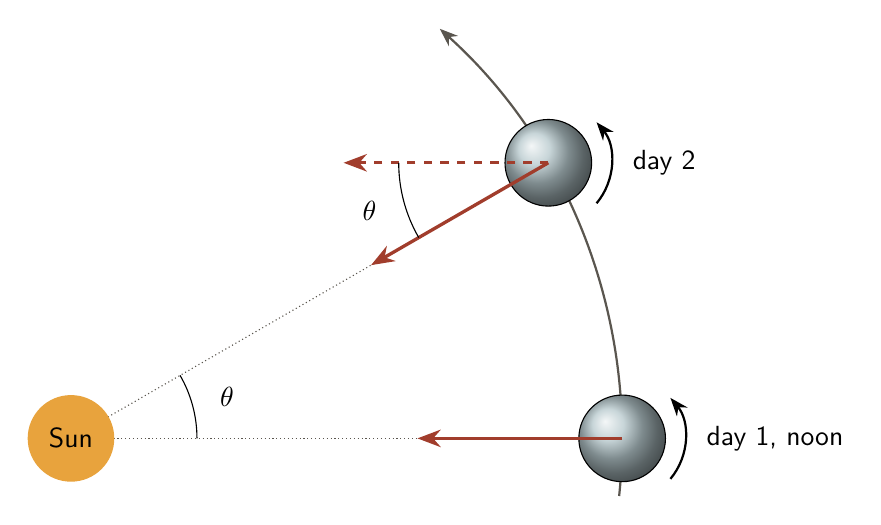
\begin{tikzpicture}[>=Stealth, font=\sffamily]
	\coordinate (S) at (0,0);
	\coordinate (E1) at (\RAD,0);
	\coordinate (E2) at (\ANG:\RAD);
	% orbit
	\draw[muted, thick, ->] (-6:\RAD) arc[start angle=-6, end angle=48, radius=\RAD];
	% Sun-Earth lines
	\draw[muted, densely dotted] (S) -- (E1);
	\draw[muted, densely dotted] (S) -- (E2);
	% Sun
	\fill[sunyellow] (S) circle (0.55);
	\node at (S) {Sun};
	% orbital angle at the Sun
	\draw (1.6,0) arc[start angle=0, end angle=\ANG, radius=1.6];
	\node at (\ANG/2:2.05) {$\theta$};
	% Earths
	\foreach \E in {E1,E2} {
		\shade[ball color=accent2!35] (\E) circle (0.55);
		\draw (\E) circle (0.55);
		\draw[->, thick] ($(\E)+(-40:0.8)$) arc[start angle=-40, end angle=40, radius=0.8];
	}
	% day 1: meridian of the observer points at the Sun
	\draw[->, very thick, accent] (E1) -- ++(180:\ARR);
	% day 2: same direction in space (dashed) and toward the Sun (solid)
	\draw[->, very thick, accent, dashed] (E2) -- ++(180:\ARR);
	\draw[->, very thick, accent] (E2) -- ++(180+\ANG:\ARR);
	% angle at Earth 2
	\draw ($(E2)+(180:1.9)$) arc[start angle=180, end angle=180+\ANG, radius=1.9];
	\node at ($(E2)+(180+\ANG/2:2.35)$) {$\theta$};
	% labels
	\node[anchor=west] at ($(E1)+(0.95,0)$) {day 1, noon};
	\node[anchor=west] at ($(E2)+(0.95,0)$) {day 2};
\end{tikzpicture}
\end{document}
